% !TEX root = ./../../_Thesis.tex

% section's Name and Label
\section{Experimental Design}
\label{subsec:ExperimentalDesign}

In order to verify the correlation between the absolute threshold and defocus,
%spherical aberration  (\ie, validate $H_{1}$ and refute $H_{0}$),
we have prepared a controlled experiment (Figure~\ref{fig:experiment}). All participants were informed about the risks, burdens, and benefits of the research. Next, all participants had their vision assessed (under the supervision of an ophthalmologist) without and with the use of cycloplegic eyedrops. First, they had their vision assessed using an autorefractor (model KR-8900, by TOPCON), which is an instrument routinely used for automatically performing objective refraction tests (\ie, estimating low-order refractive errors).  
Then, each subject received one drop of a cycloplegic eyedrops 
%\review{(temos nome do que foi usado?)} 
in each of the eyes, and after 15 minutes, the autorefractor test was repeated. A {\it cycloplegic drug} relaxes the ciliary muscles, which are responsible for allowing the eye to focus at different distances. A cycloplegic drug can be used to relax the ciliary muscles (\ie, avoid accommodation), forcing the eye to focus at infinity. Complete relaxation, however, requires relatively-high concentrations of the drug.
%
\begin{figure}[htb]
	\centering
	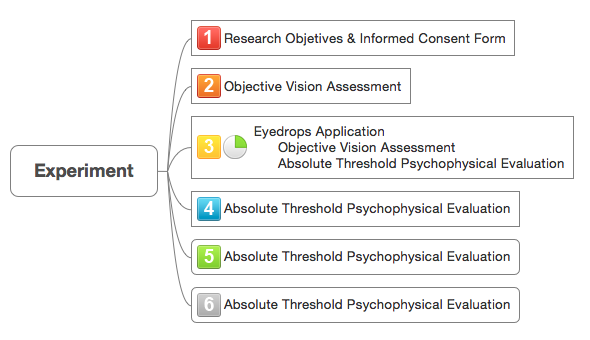
\includegraphics[width=1.0\linewidth]{__Images/04/experiment.png}
	\caption[Stages of the Absolute Threshold experiment]{Stages of the Absolute Threshold experiment.}
	\label{fig:experiment}
\end{figure}

For the psychophysical experiment, each subject performed four  evaluations to establish his/her absolute threshold for vision. The first psychophysical evaluation was applied right after the second objective vision assessment (under the effect of the cycloplegic eyedrops). The other three evaluations were taken with intervals of at least one day between each other. 

%To achieve a statistically reliable estimate 
All evaluations were performed with naked eye (\ie, the subject were not allowed to use corrective eyeglasses or contact lenses). 
To obtain a larger and uniformly-distributed sample set, each eye of each subject was tested 17 times simulating various degrees of refractive errors. For this, we added to the apparatus external lenses with integer powers ranging from -5.0 D $\hdots$ 0.0 D $\hdots$ +5.0 D, as well as $\pm$0.25 D, $\pm$0.5 D, and $\pm$1.5 D (Figure~\ref{fig:apparatus_with_extra_lens}). The net effect is summing these powers to the original refractive errors of the participants. Between any two tests, there was an interval of approximately thirty seconds.
%a total of  
%we have added extra lenses to  the device used in the psychophysical evaluations. Thus, for each evaluation of each subject, we used 16 additional lenses with integer powers ranging from -5.0 D to +5.0 D, as well as $\pm$0.25 D, $\pm$0.5 D, and $\pm$1.5 D. 
The order in which the lenses were placed in the device was randomly defined for each subject. 
A detailed description of the apparatus is presented in Section~\ref{sec:Apparatus_and_Measurements}, and more details about the experiments are provided 
%Avoiding accommodation process was target by randomizing the extra lenses order. This order, as well as other information, are described 
in Appendix \ref{chap:AppendixA}.

\begin{figure}[!htb]
	\centering
		\subfigure[]{
		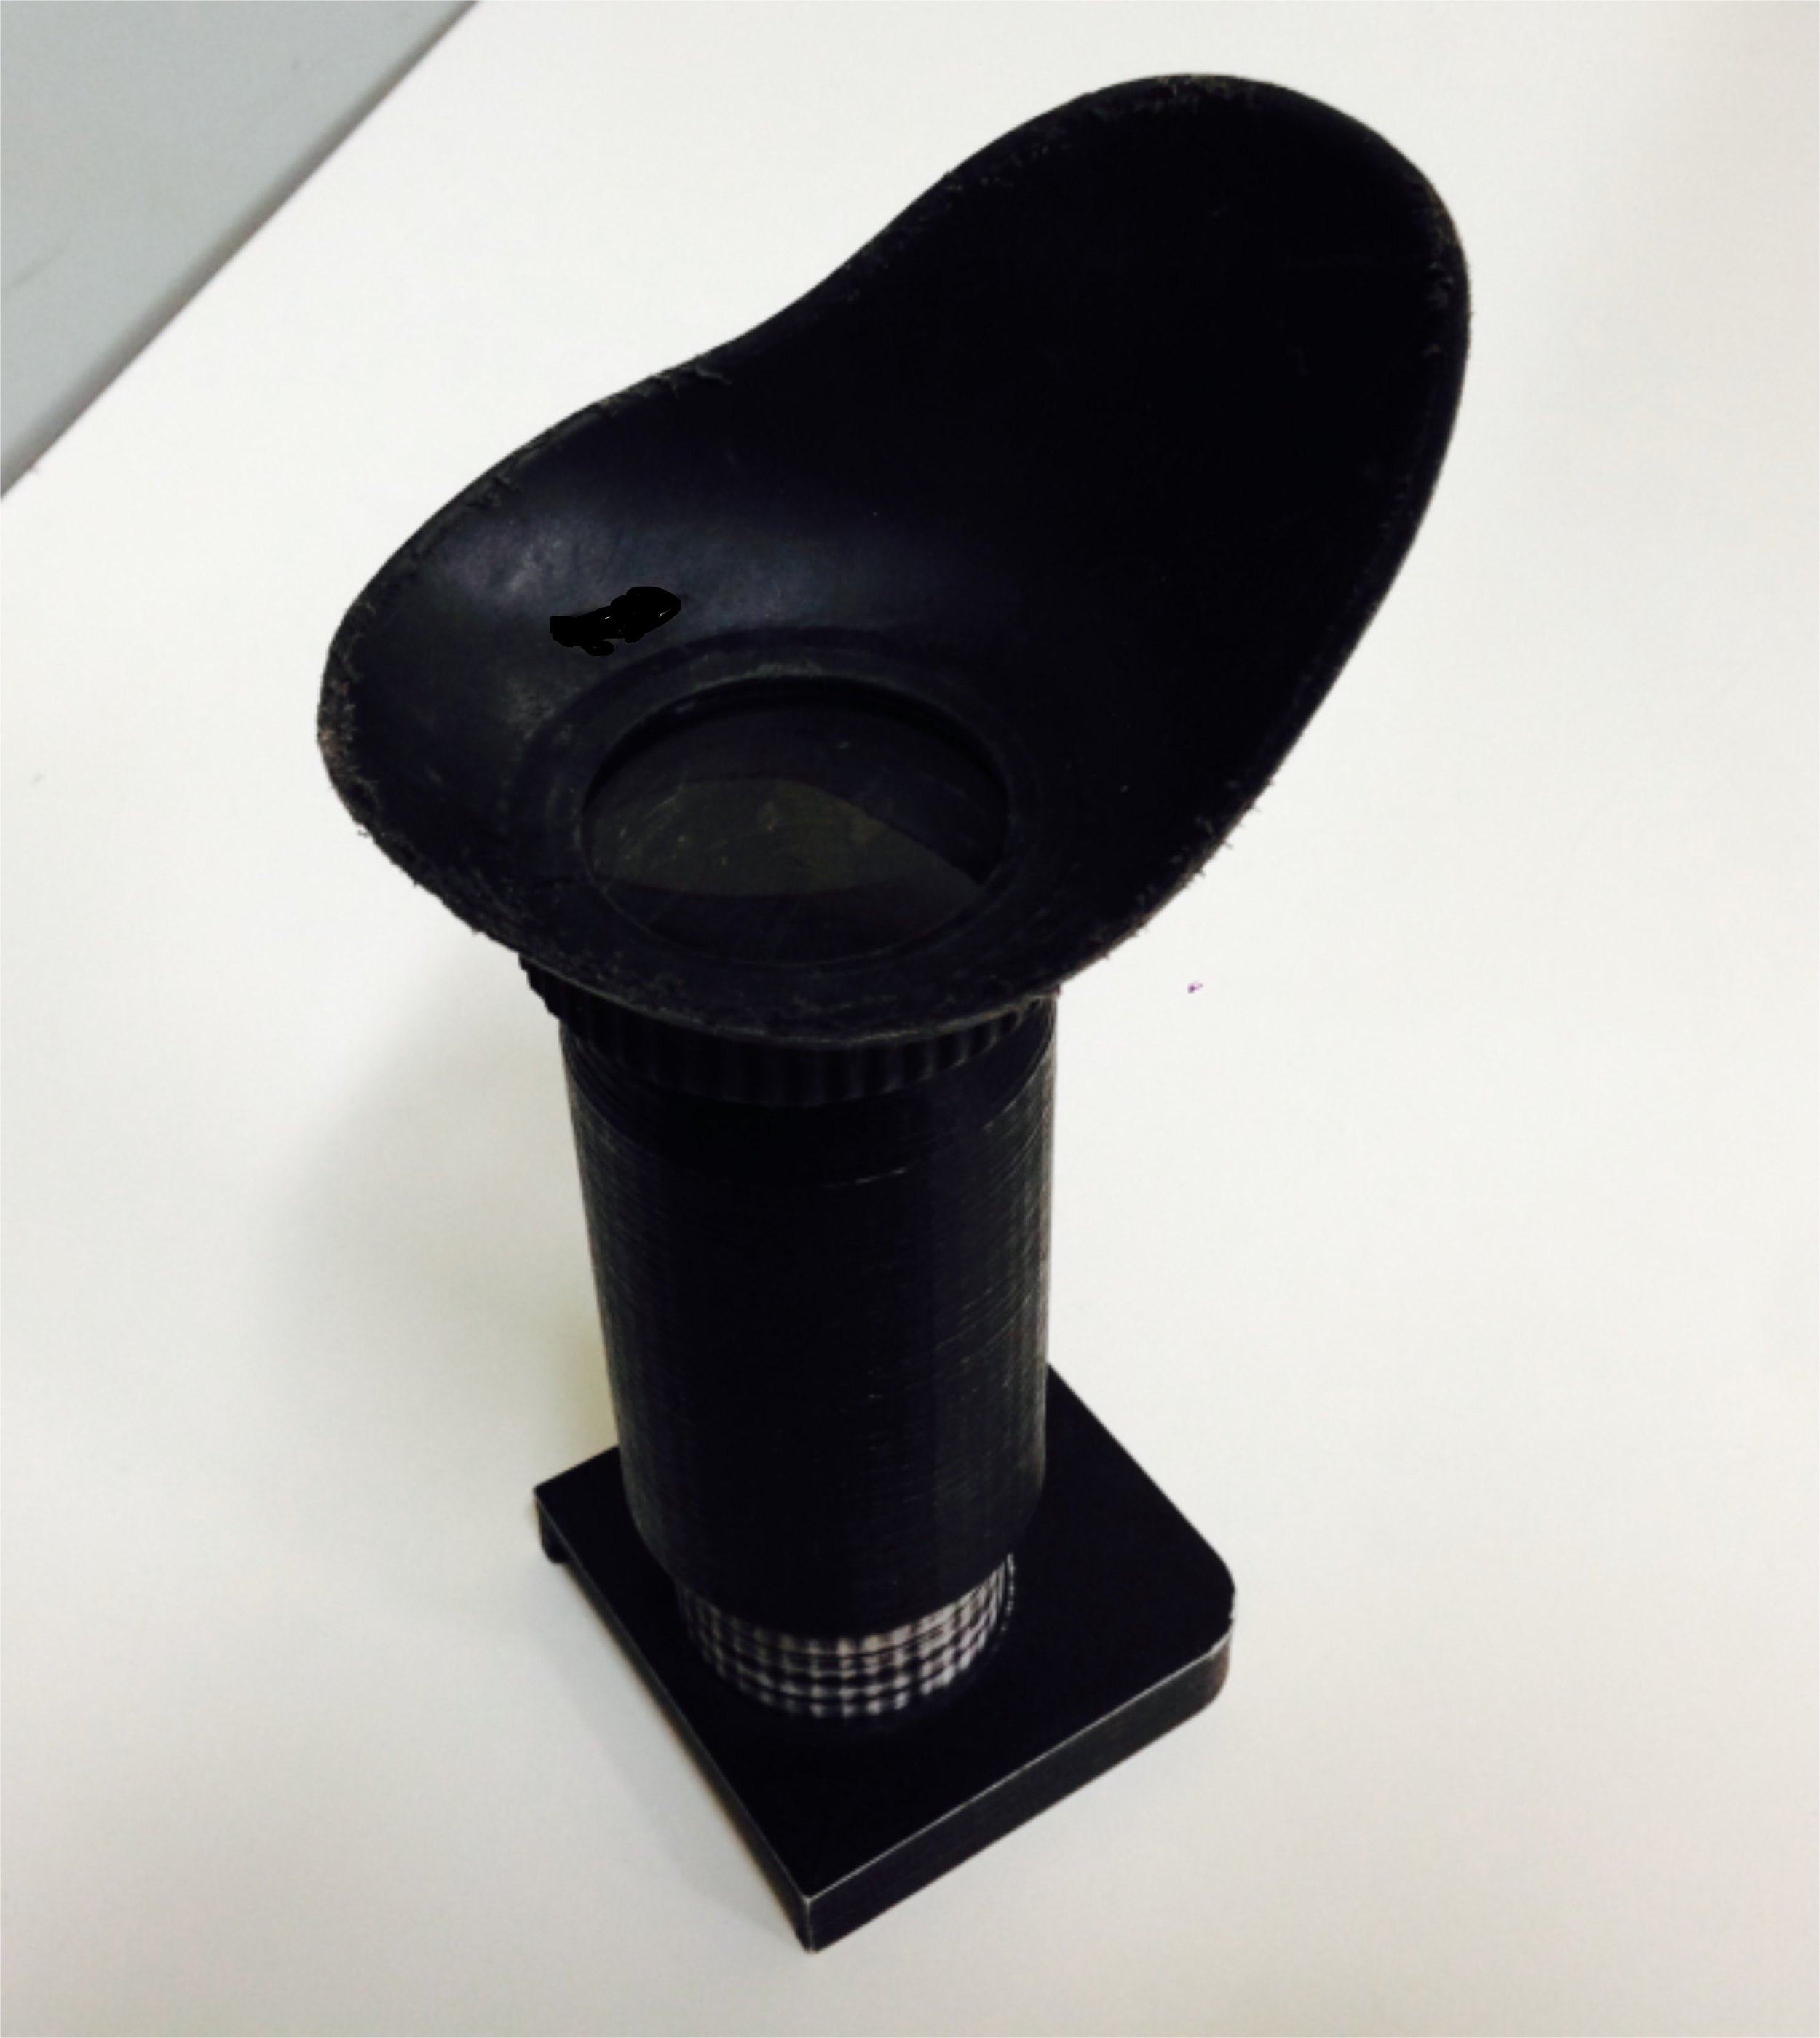
\includegraphics[width=0.3\linewidth]{__Images/05/52/without_lens.png}
		\label{fig:prot}
	}
	\subfigure[]{
		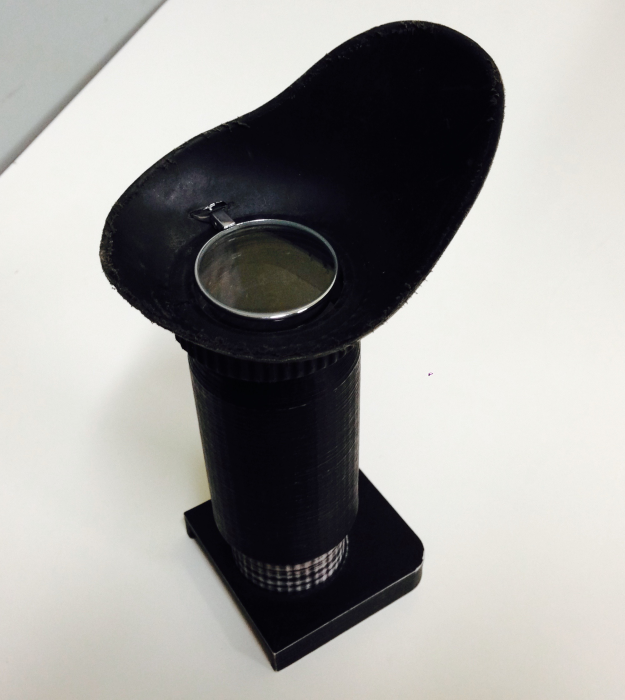
\includegraphics[width=0.3\linewidth]{__Images/05/52/with_lens.png}
		\label{fig:prot_with_lens}
	}
	\subfigure[]{
		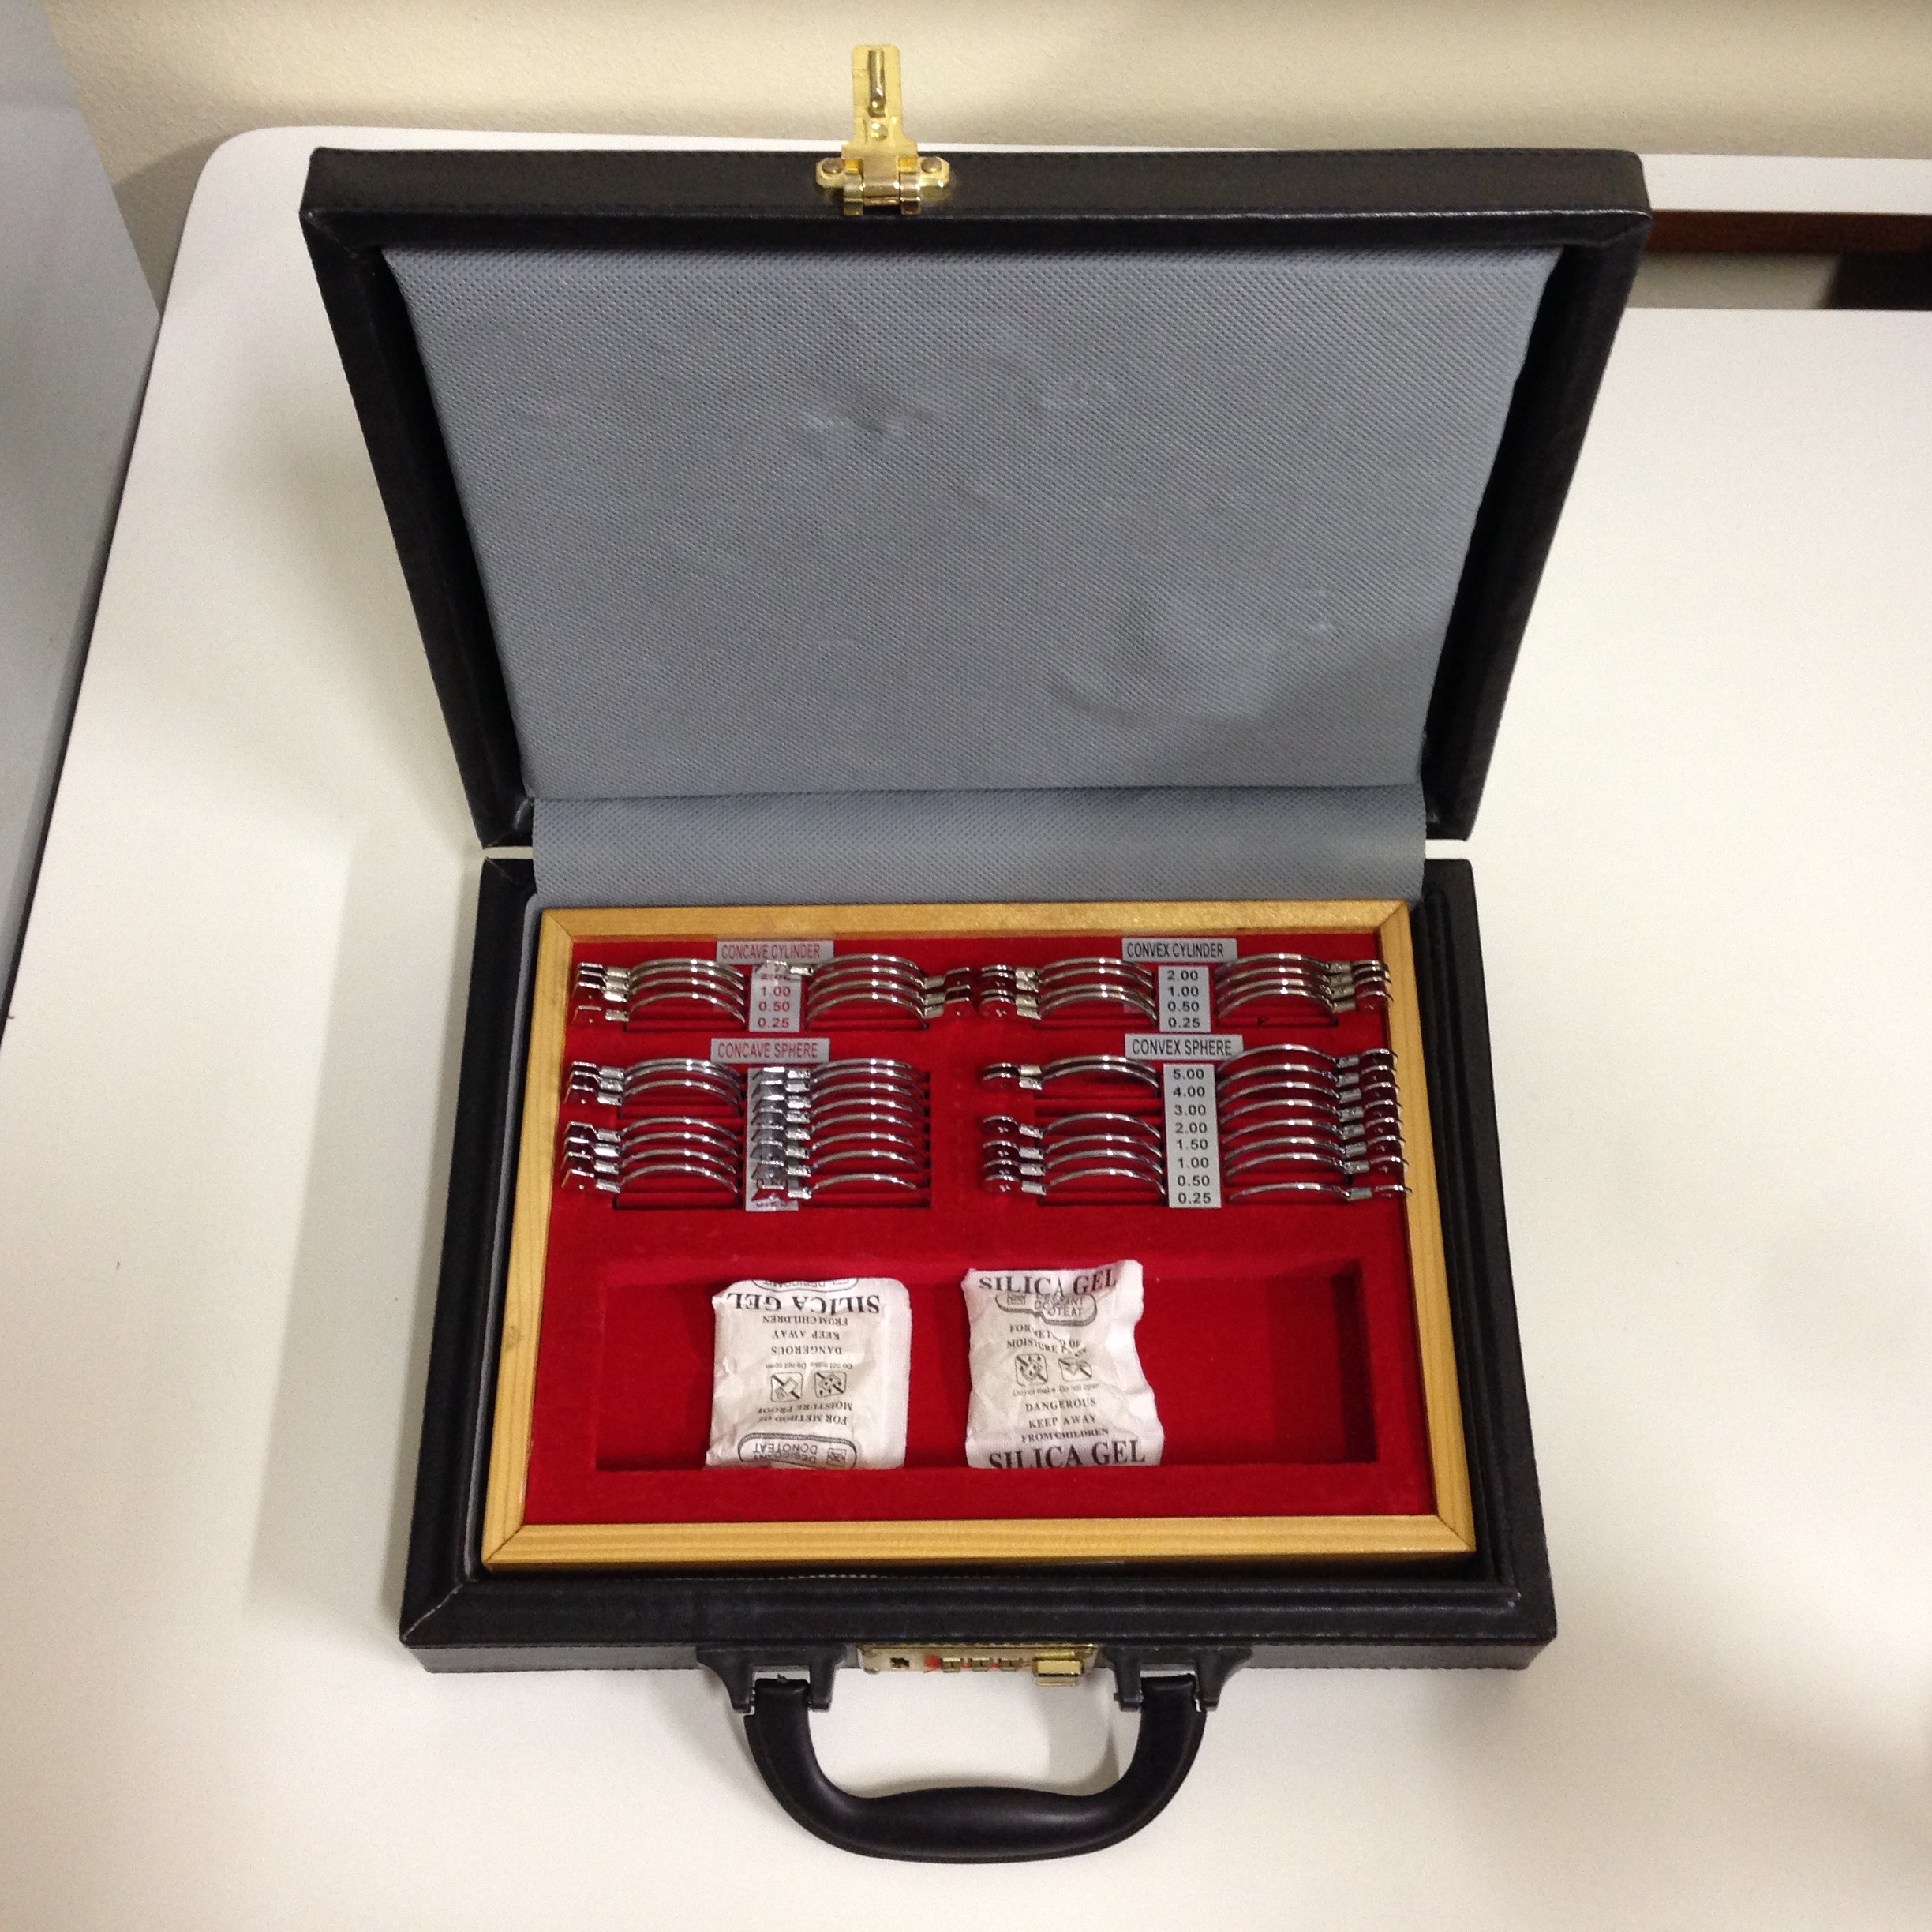
\includegraphics[width=0.3\linewidth]{__Images/05/52/lensset.jpg}
		\label{fig:trial_lens_set}
	}
	\caption[Apparatus designed for the psychophysical experiment]{Apparatus designed for the psychophysical experiment. (a) Apparatus. (b) Apparatus showing an additional lens. (c) Trial lens set containing lenses with various dioptric powers used for the experiment.}
	\label{fig:apparatus_with_extra_lens}
\end{figure}

